
\documentclass[11pt]{article}

\usepackage{fullpage,epsfig,latexsym,picinpar,amsbsy,amsmath,tikz}


\setlength{\evensidemargin}{0.1in}
\setlength{\oddsidemargin}{0.1in}
\setlength{\textwidth}{6.6in}
\setlength{\topmargin}{0.0in}
\setlength{\textheight}{8.7in}
\setlength{\headheight}{0in}
\setlength{\headsep}{0in}
\setlength{\topsep}{0in}
\setlength{\itemsep}{0in}
\renewcommand{\baselinestretch}{1.1}
\parskip=0.080in
                                                                                                                         
\newcommand{\parend}[1]{{\left( #1  \right) }}
\newcommand{\spparend}[1]{{\left(\, #1  \,\right) }}
\newcommand{\angled}[1]{{\left\langle #1  \right\rangle }}
\newcommand{\brackd}[1]{{\left[ #1  \right] }}
\newcommand{\spbrackd}[1]{{\left[\, #1  \,\right] }}
\newcommand{\braced}[1]{{\left\{ #1  \right\} }}
\newcommand{\leftbraced}[1]{{\left\{ #1  \right. }}
\newcommand{\floor}[1]{{\left\lfloor #1\right\rfloor}}
\newcommand{\ceiling}[1]{{\left\lceil #1\right\rceil}}
\newcommand{\barred}[1]{{\left|#1\right|}}
\newcommand{\doublebarred}[1]{{\left|\left|#1\right|\right|}}
\newcommand{\spaced}[1]{{\, #1\, }}
\newcommand{\suchthat}{{\spaced{|}}}
\newcommand{\numof}{{\sharp}}
\newcommand{\assign}{{\,\leftarrow\,}}
                                                                                                                         
\newcommand{\veps}{{\varepsilon}}
\newcommand{\Sigmastar}{{\Sigma^\ast}}
\newcommand{\barx}{{ \bar x}}

\newcommand{\half}{{\mbox{$\frac{1}{2}$}}}
\newcommand{\threehalfs}{{\mbox{$\frac{3}{2}$}}}





\newcommand{\Union}{\mbox{\rm Union}}
\newcommand{\Find}{\mbox{\rm Find-Set}}

\newcommand{\delete}{{\mbox{\tt delete}}}
\newcommand{\decreasekey}{{\mbox{\tt decreasekey}}}
\newcommand{\extractmin}{{\mbox{\tt extractmin}}}

\pagestyle{empty}
\begin{document}

\centerline{\large \bf CS218 ASSIGNMENT 2}
\centerline{due Thursday, February~7, at 5PM}

\vskip 0.1in
\noindent
{\bf Individual assignment: Problems 1,2}

\noindent
{\bf Group assignment: Problems 1,2,3}

\vskip 0.1in

%%%%%%%%%%%%%%%%%%%%%%%%%%%%

\begin{problem}
Consider Fibonacci heap $H$ below. Marked vertices are designated
with double circles. Apply the following sequence of operations to $H$:
$\decreasekey(H,x,11)$, $\delete(H,y)$, $\extractmin(H)$. Draw $H$
after each operation.

\noindent
\begin{center}
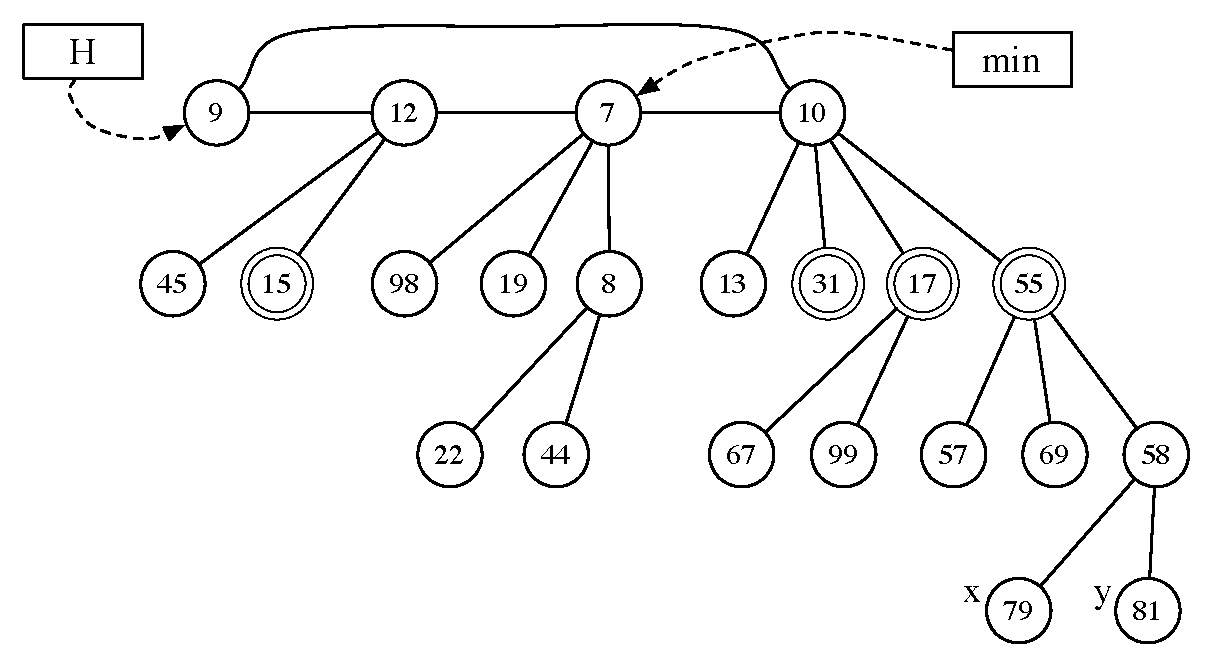
\includegraphics[width=4.25in]{hw2_fib_heap.pdf} %
\end{center}

\end{problem}

\paragraph{Answer}
\tikzset {
    treenode/.style={align=center,inner sep=0pt},
    % black nodes
    node_black/.style={treenode,circle,white,font=\bfseries,draw=black,fill=black,text width=0.6cm},
    % white nodes
    node_white/.style={treenode,,circle,draw=black,text width=0.6cm},
    % triangle
    triangle/.style = {regular polygon, regular polygon sides=3 }
}
After $\decreasekey(H,x,11)$, we mark the node of $key=58$. The $min$ pointer is unchanged.

\begin{tikzpicture}
%[->,level/.style = {sibling distance=2cm, level distance=1.5cm}]
\node[node_white] at (0,0) (A){9};
\node[node_white] at (3,0) (B){12}
    child{ node[node_white] at (-1,0) (C){45} }
    child{ node[node_black] at (-1,0) (D){15} };
\node[node_white] at (6,0) (E) {7}
    child{ node[node_white] at (-0.8,0) (F){98} }
    child{ node[node_white] at (-0.8,0) (G){19} }
    child{ node[node_white] at (-1,0) (H){8} 
        child{ node[node_white] at (-1,0) (I){22} }
        child{ node[node_white] at (-1,0) (J){44} }
    };
\node[node_white] at (9,0) (L) {10}
    child{ node[node_white] at (0.8,0) (M){13} }
    child{ node[node_black] at (0.8,0) (N){31} }
    child{ node[node_black] at (0.8,0) (O){17} 
        child{ node[node_white] at (-1,0) (Q){67} }
        child{ node[node_white] at (-1,0) (R){99} }
    }
    child{ node[node_black] at (0.8,0) (P){55} 
        child{ node[node_white] at (0.8,0) (S){57} }
        child{ node[node_white] at (0.5,0)(T){69} }
        child{ node[node_black] at (0.2,0) (U){58} 
            child{ node[node_white] (W){81} }
        }
    };
\node[node_white] at (12,0) (V){11};

\draw[] (A) -- (B);
\draw[] (B) -- (E);
\draw[] (E) -- (L);
\draw[] (L) -- (V);

\end{tikzpicture}

After $\delete(H,y)$, we need to do a cascade cut for both the parent and grandparent of $y$. The $min$ pointer is unchanged.

\begin{tikzpicture}
%[->,level/.style = {sibling distance=2cm, level distance=1.5cm}]
\node[node_white] at (0,0) (A){9};
\node[node_white] at (2,0) (B){12}
    child{ node[node_white] at (-1,0) (C){45} }
    child{ node[node_black] at (-1,0) (D){15} };
\node[node_white] at (5,0) (E) {7}
    child{ node[node_white] at (-0.8,0) (F){98} }
    child{ node[node_white] at (-0.8,0) (G){19} }
    child{ node[node_white] at (-1,0) (H){8} 
        child{ node[node_white] at (-1,0) (I){22} }
        child{ node[node_white] at (-1,0) (J){44} }
    };
\node[node_white] at (8,0) (L) {10}
    child{ node[node_white] at (0.8,0) (M){13} }
    child{ node[node_black] at (0.8,0) (N){31} }
    child{ node[node_black] at (0.8,0) (O){17} 
        child{ node[node_white] at (-1,0) (Q){67} }
        child{ node[node_white] at (-1,0) (R){99} }
    };
\node[node_white] at (11,0) (V){11};
\node[node_black] at (13,0) (U){58};
\node[node_black] at (15,0) (P){55} 
        child{ node[node_white] at (0,0) (S){57} }
        child{ node[node_white] at (0,0) (T){69} };
        
\draw[] (A) -- (B);
\draw[] (B) -- (E);
\draw[] (E) -- (L);
\draw[] (L) -- (V);
\draw[] (V) -- (U);
\draw[] (U) -- (P);
\end{tikzpicture}

On $\extractmin(H)$, we remove the node of $key=7$ from the root list, and append all its sub-tree to the list, then do $union$. And the $min$ is pointing to the node of $key=9$.

\begin{tikzpicture}
%[->,level/.style = {sibling distance=2cm, level distance=1.5cm}]
\node[node_white] at (0,0) (A){19};
\node[node_white] at (3,0) (B){55}
    child{ node[node_white] at (-1,0) (C){57} }
    child{ node[node_black] at (-1,0) (D){69} };
\node[node_white] at (6,0) (E) {9}
    child{ node[node_white] at (-0.8,0) (F){11} }
    child{ node[node_white] at (-1,0) (G){58} 
        child{ node[node_white] (H){98} }
    };
\node[node_white] at (9,0) (I) {8}
    child{ node[node_white] (J){22} }
    child{ node[node_white] (K){44} }
    child{ node[node_white] (L){12} 
        child{ node[node_black] at (-1,0) (M){15} }
        child{ node[node_white] at (-1,0) (N){45} }
    }
    child{ node[node_white] (O){10}
        child{ node[node_white] at (1,0) (P){13} }
        child{ node[node_black] at (1,0) (Q){31} }
        child{ node[node_black] at (1,0) (R){17} 
            child{ node[node_white] (S){67} }
            child{ node[node_white] (T){99} }
        }
    };
    
\draw[] (A) -- (B);
\draw[] (B) -- (E);
\draw[] (E) -- (I);

\end{tikzpicture}


%%%%%%%%%%%%%%%%%%%%%%%%%%%%

\newcommand{\cost}{{\mbox{\it cost}}}

\begin{problem}
When analyzing the amortized cost of the ziggy operations,
in Lemma~1b,
we proved that $\partial\cost + \partial\Phi \le 3\partial\omega_x$
holds for (Zig-Zig). Prove that the same inequality
holds for (Zig-Zag).
\end{problem}

\paragraph{Answer}
In Zig-Zag case, we have $\omega'(x) = \omega(z)$, $\omega'(y) \leq \omega'(x)$, $\omega(x) \leq \omega(y) \leq \omega(z)$, $\omega'(z) \leq \omega'(x)$, and all the other weight keep unchanged.
To maintain the invariant we need:
\begin{gather*}
    \partial\Phi = \partial\omega(x) + \partial\omega(y) + \partial\omega(z) = \omega'(x) + \omega'(y) + \omega'(z) - \omega(x) - \omega(y) - \omega(z) \\
    \partial\Phi + \partial cost = \partial\omega(x) + \partial\omega(y) + \partial\omega(z) + 2 \\ 
    = 2 + \partial\omega(x) + \omega'(y) - \omega(y) + \omega'(z) - \omega(z) \\
    \leq 2 + \partial\omega(x) + \omega'(x) - \omega(x) + \omega'(z) - \omega(z) \\
    = 3\partial\omega(x) + [2 - 2\omega'(x) + \omega'(z) + \omega(x)]
\end{gather*}
We need to prove that $2 - 2\omega'(x) + \omega'(z) + \omega(x) \leq 0$.

% \noindent
% \begin{center}
% 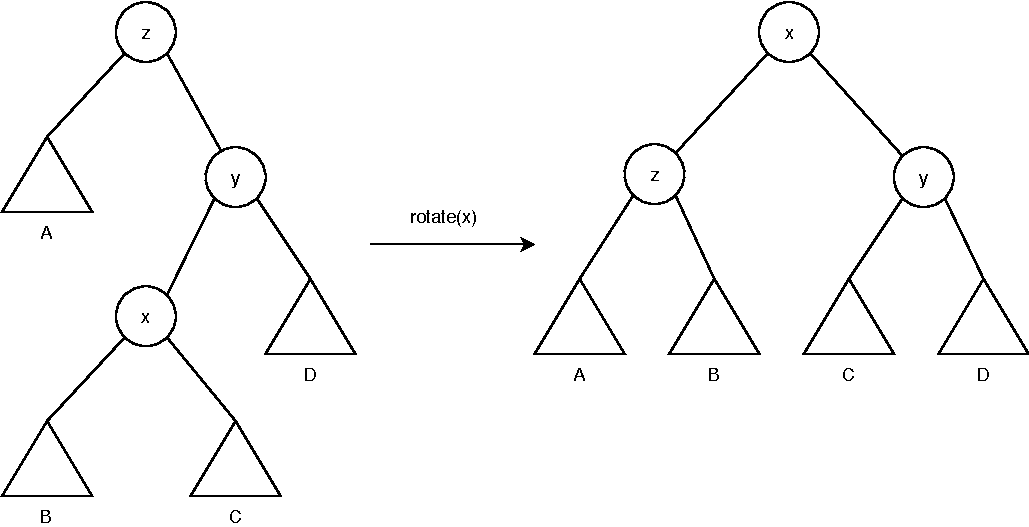
\includegraphics[width=4in]{hw2_2.pdf} %
% \end{center}
\begin{tikzpicture}
\node[node_white] {z}
    child { node[triangle] {A} }
    child { node[node_white] {y}
        child { node[node_white] {x} 
            child { node[triangle] {B} }
            child { node[triangle] {C} }
        }
        child { node[triangle] {D} }
    };
\draw[-latex] (2,-2) node[above,xshift=1cm] {Zig-Zag} -- (4,-2);
\node[node_white] at (7,0) {x} 
    child { node[node_white] at (-0.5,0) {z} 
        child { node[triangle] {A} }
        child { node[triangle] {B} }
    }
    child { node[node_white] at (0.5,0) {y} 
        child { node[triangle] {C} }
        child { node[triangle] {D} }
    };
\end{tikzpicture}

From the figure above, we have: $|T_x| = |B| + |C|$, $|T_z'| = |A| + |B|$, and $|T_x'| = |A| + |B| + |C| + |D| + z' + y'$, then we get  $|T_x| + |T_z| \leq |T_x'|$.
Supposing $2 - 2\cdot\omega'(x) + \omega'(z) + \omega(x) \leq 0$ is true:
\begin{gather*}
    2 - 2\omega'(x) + \omega'(z) + \omega(x) \leq 0\\
    2 - 2 \cdot log|T_x'| + log|T_z'| + log|T_x| \leq 0 \\
    4 \cdot \frac{|T_z'||T_x|}{|T_x'|^2} \leq 1
\end{gather*}
As long as we have $|T_x| + |T_z| \leq |T_x'|$, the inequality is true.
Therefore, in Zig-Zag, we also have $\partial\Phi + \partial cost \leq 3 \partial\omega(x)$.

%%%%%%%%%%%%%%%%%%%%%%%%%%%%

\begin{problem}
Suppose that we start with the following splay tree (with keys
ordered alphabetically):
%
\noindent
\begin{center}
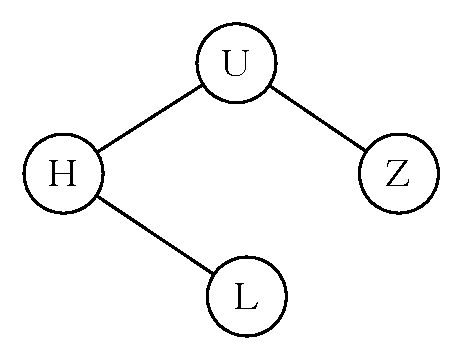
\includegraphics[width=1.75in]{hw2_splay_tree.pdf} %
\end{center}
%
and then we insert the keys
$F, S, Q, W, R, A, D$,
and then delete $ Q, S$.
Draw the tree
(a) after inserting $W$, (b) after inserting $D$,
(c) after deleting $S$.
\end{problem}

\paragraph{Answer}
(a) After inserting $W$:

\begin{tikzpicture}
\node[node_white] {W}
    child{ node[node_white] {Q} 
        child{ node[node_white] {L}
            child{ node[node_white] at (-0.8,0) {F}
                child{ node[node_white] at (0.8,0) {H} }
            }
        }
        child{ node[node_white] {U}
            child{ node[node_white] at (-0.8,0) {S} }
        }
    }
    child{ node[node_white] {Z} };
\end{tikzpicture}

(b) After inserting $D$:

\begin{tikzpicture}
\node[node_white] {D}
    child{ node[node_white] {A} }
    child{ node[node_white] {F}
        child { node[node_white] at (0.8,0) {R}
            child { node[node_white] {L}
                child { node[node_white] {H} }
                child { node[node_white] {Q} }
            }
            child { node[node_white] {S}
                child { node[node_white] at (0.8,0) {W} 
                    child { node[node_white] {U} }
                    child { node[node_white] {Z} }
                }
            }
        }
    };
\end{tikzpicture}

(c) After deleting $S$:

\begin{tikzpicture}
\node[node_white] {R}
    child { node[node_white] {L} 
        child { node[node_white] at (-0.8,0) {D}
            child { node[node_white] {A} }
            child { node[node_white] {H} 
                child { node[node_white] at (-0.8,0) {F} }
            }
        }
    }
    child { node[node_white] {W} 
        child { node[node_white] {U} }
        child { node[node_white] {Z} }
    };
    
\end{tikzpicture}

%%%%%%%%%%%%%%%%%%%%%%%%%%%%

\vskip 0.2in
\paragraph{Submission.}
Submit the pdf file via gradescope by 5PM on Thursday, February~7.
For pair assignments, submit one pdf only with two names on it.


\end{document}

